%!TEX root = ../dokumentation.tex

\chapter{Planung}\label{cha:Planung}
Bevor mit die Entwicklung der Anwendung begonnen werden kann, müssen die Anforderungen, sowie Ziele und Umgebung festgelegt werden. Die exakte Planung eines ist notwendig, um eine qualitativ hochwertige, lösungsorientierte Anwendung zu entwickeln.

%Beschreiben worum es im Kapitel geht. Warum wird eine Planung gemacht? Was ist das Ziel der Planung?

\section{Ermittlung der Anforderungen}
<Kreative Beschreibung der Anforderungen. Was soll das Programm am ende können? Welche Bedingungen gibt es? Welche Limits hat es? Hier ist wichtig das die Anforderungen noch keine Ziele sind. Es geht nur darum zu ermitteln was abgedeckt sein muss.>

\section{Formulierung konkreter Ziele}
<In diesem Kapitel sollen die Anforderungen in konkrete Ziele überführt werden. Diese müssen SMART sein, damit sie später bei einem Abgleich verwendet werden können.>

\section{Definition der Umgebung}
Die Programmierung der Anwendung erfolgt in der Programmiersprache Java, unter verwendung des Hadoop Frameworks für MapReduce in der Version 2.7.1. Die Entwicklung wird mit der \ac{IDE} \gls{NetBeans}, Version 8.0.2, durchgeführt. Für die Versionsverwaltung wird \gls{Git} eingesetzt. In der \ac{IDE} wird ein \gls{Maven}-Projekt erzeugt, um alle benötigten Bibliotheken automatisch, durch die \ac{IDE}, beziehen zu können.

%TODO: Datenbank definieren
Über die \ac{IDE} wird eine ausführtbare JAR-Datei erzeugt, welche auf dem Server mit Hadoop ausgeführt werden soll. Für die Ausführung wird Java in Version 1.7 benötigt. Zusätzlich wird eine <PUTNAM> Datenbank für die Speicheurng der Ausgabe benötigt.

Die anwendung wird durch das Hadoop Framework Version 2.7.1 ausgeführt. Es muss mindestens eine \textit{Single Node} Installation vorhanden sein. Es müssen die entsprechenden Rechte auf dem Dateisystem \ac{HDFS} gesetzt sein, um Dateien lesen und schreiben zu können.

%Welche Sprache wird verwendet? Auf welcher Plattform wird entwickelt? Welche Technologien werden eingesetzt.

\section{Datenschutzrichtlinien}
<Hier müssen die Datenschutzbestimmungen abgehandelt werden. Im normalfall wären IP Adressen personenbezogene daten und müssten geschützt werden. Es gibt da aber die außnahme in verbindung mit dem gesetz zur Vorratsdatenspeicherung. Darauf muss eingegangen werden um klar zu stellen unter welchen rechtlichen grundlagen die verarbeitung hier stattfinden kann. Dabei sollten auch die begriffe der anonymisierung und pseudonymisierung geklärt werden und was gemacht werden muss (wenn überhaupt).>

\section{Verarbeitungsprozess}
<Hier sollte der Prozess der Anwendung geplant werden. wo liegen die Daten? wie findet der zugriff statt? nach welchem schema sind sie abgelegt und benannt? Außerdem sollte klar werden wie die Informationen verarbeitet werden. ein großer map reduce oder eine verkettung mehrerer mapper und reducer? Außerdem muss das ausgabeformat festgelegt werden. Bzw. zwei alternativen. eine für wenn die anwendung performant genug ist um als check skript zu laufen, und eine für den fall das nicht.>

\begin{figure}
	\centering
	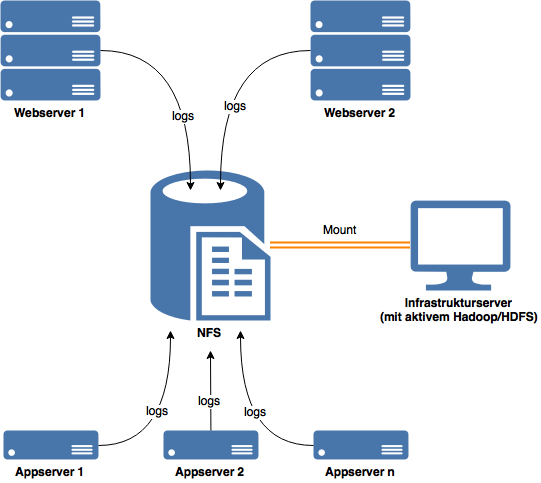
\includegraphics[width=.8\textwidth]{Infrastruktur.png}
	\caption{DUMMY: Aufbau der Infrastruktur}
	\label{fig:AufbauInfrastruktur}
\end{figure}